%%%%%%%% CIL 2026 PROJECT REPORT %%%%%%%%%%%%%%%%%%%%%%%%%%%%%%%%%%%%%%%%%%%%%%%%

\documentclass{article}

\usepackage{microtype}
\usepackage{graphicx}
\usepackage{subfigure}
\usepackage{booktabs}
\usepackage{hyperref}
\usepackage{amsmath}
\usepackage{amssymb}
\usepackage{mathtools}
\usepackage{amsthm}
\usepackage{enumitem}
\usepackage{xcolor}
\usepackage[capitalize,noabbrev]{cleveref}
\usepackage[accepted]{icml2024}
\usepackage{placeins}   % \FloatBarrier — keeps floats within their section
\usepackage{multirow}   % \multirow in tables
\usepackage{float}      % [H] float placement

\newcommand{\TODO}[1]{\textcolor{red}{\textbf{[TODO: #1]}}}
\newcommand{\KP}[1]{\textit{#1}}   % keypoint — rendered as italic

\icmltitlerunning{Ordinal Sentiment Classification via Wasserstein Loss and Cross-Validation Ensembling}

\begin{document}

\twocolumn[
\icmltitle{Ordinal Sentiment Classification via\\
           Wasserstein Loss, Median Decoding,\\
           and Cross-Validation Ensembling}

\icmlsetsymbol{equal}{*}

\begin{icmlauthorlist}
\icmlauthor{\TODO{Author 1}}{eth}
\icmlauthor{\TODO{Author 2}}{eth}
\icmlauthor{\TODO{Author 3}}{eth}
\end{icmlauthorlist}

\icmlaffiliation{eth}{Department of Computer Science, ETH Zürich, Switzerland}

\icmlkeywords{ordinal regression, sentiment analysis, Wasserstein loss, transformer fine-tuning}

\vskip 0.3in
]

\printAffiliationsAndNotice{\icmlEqualContribution}

% ─────────────────────────────────────────────────────────────────────────────
\begin{abstract}
\TODO{Write abstract. Mention: task (ordinal sentiment 1-5 stars), metric
(1-MAE/4), approach (W2 loss + median decode + mDeBERTa + LLRD + EMA +
seed-split ensemble), final score (0.9078).}
\end{abstract}

% ─────────────────────────────────────────────────────────────────────────────
\section{Introduction}
\label{sec:intro}

\begin{itemize}[leftmargin=*,itemsep=1pt]
  \item Task: 5-class ordinal sentiment (1--5 stars), metric $= 1 - \text{MAE}/4$
  \item Ordinal $\neq$ classification: class distances matter;
        predicting 1 when truth is 5 is strictly worse than predicting 4
  \item Standard cross-entropy treats all misclassifications equally ---
        ignores ordinal structure
  \item \textbf{Central thesis:} the CDF of the predicted class distribution
        unifies loss (W$^2$), decoding (median), and evaluation (MAE) into
        one coherent geometric framework
  \item Preview of result: 0.9078 test score, new best achieved by
        mDeBERTa-v3 + LLRD + EMA + 3-seed independent-split ensemble
\end{itemize}

\TODO{Write introduction text}

% ─────────────────────────────────────────────────────────────────────────────
\section{Related Work}
\label{sec:related}

\begin{itemize}[leftmargin=*,itemsep=1pt]
  \item Ordinal regression losses: CORAL (pairwise binary thresholds),
        SORD (KL against soft targets), Wasserstein/EMD-based
  \item mDeBERTa-v3: disentangled attention over content + position,
        278M params, multilingual pretraining on 100 languages
  \item Catastrophic forgetting in fine-tuning: motivation for LLRD
  \item EMA for smoother generalisation in deep networks
  \item Cross-validation ensembling vs.\ seed ensembling
\end{itemize}

\TODO{Write related work text}

% ─────────────────────────────────────────────────────────────────────────────
\section{Method}
\label{sec:method}

\subsection{The Elegant Core: CDF as Unifying Object}

\begin{itemize}[leftmargin=*,itemsep=1pt]
  \item \KP{The same object --- the predicted CDF $\hat{F}(k) = \sum_{j \leq k} p_j$
        --- appears in the loss, the decoder, and the evaluation metric.}
  \item \KP{Loss:} W$^2$ penalises the squared $L_2$ distance between
        predicted CDF and true CDF (a step at the true class)
  \item \KP{Decoder:} median = first $k$ where $\hat{F}(k) \geq 0.5$;
        Bayes-optimal under MAE
  \item \KP{Metric:} MAE is minimised by the median of the predictive distribution
  \item This is principled, not heuristic: loss, decoder, and metric
        all express the same ordinal geometry
\end{itemize}

\subsection{Wasserstein$^2$ Loss}
\label{sec:emd}

\begin{itemize}[leftmargin=*,itemsep=1pt]
  \item Wasserstein-1 for discrete distributions (Earth Mover's Distance)
  \item Closed form: squared $L_2$ distance between predicted and true CDFs
  \item Why squared: smooth gradients; larger distributional errors penalised more
  \item CE only sees the true class; W$^2$ propagates gradient through all
        class probabilities
  \item SORD (KL divergence): failed completely --- stuck at 0.8527,
        model collapsed to near-uniform distributions
  \item CORAL (pairwise binary): 0.8576 --- ordinal geometry less direct
\end{itemize}

\begin{equation}
  \mathcal{L}_{W^2}(\mathbf{p}, y)
  = \sum_{k=0}^{K-2} \Bigl(\hat{F}(k) - \mathbf{1}[k \geq y]\Bigr)^{2},
  \quad \hat{F}(k) = \textstyle\sum_{j=0}^{k} p_j
  \label{eq:w2}
\end{equation}

\TODO{Write W$^2$ loss text}

\subsection{Median Decoding}

\begin{itemize}[leftmargin=*,itemsep=1pt]
  \item $\hat{y} = \min\{k : \hat{F}(k) \geq 0.5\}$
  \item Bayes-optimal under MAE: the median minimises
        $\mathbb{E}[|y - \hat{y}|]$
  \item Argmax is Bayes-optimal for 0/1 loss, not MAE
  \item EV decode: non-integer output, failed empirically with SORD
\end{itemize}

\begin{equation}
  \hat{y} = \min\bigl\{k \in \{0,\ldots,K{-}1\} : \hat{F}(k) \geq 0.5\bigr\}
  \label{eq:median}
\end{equation}

\TODO{Write median decoding text}

\subsection{Architecture}

\begin{itemize}[leftmargin=*,itemsep=1pt]
  \item mDeBERTa-v3-base encoder (278M params)
  \item Mean pooling over all non-padding tokens (captures full review signal;
        outperforms [CLS] pooling)
  \item Multi-sample dropout (MSD): $K{=}5$ independent masks, logits averaged;
        lightweight within-model regularisation
  \item Linear head: $768 \to 5$ logits
\end{itemize}

\TODO{Write architecture text}

\subsection{Fine-Tuning: LLRD + EMA}

\begin{itemize}[leftmargin=*,itemsep=1pt]
  \item \textbf{LLRD} --- head: $5{\times}10^{-5}$; top encoder layer:
        $8{\times}10^{-6}$; decay $\times 0.9$/layer; embeddings
        $\approx\!1{\times}10^{-6}$
  \item Without LLRD (baselines 19, 20): val score peaks epoch 3 and
        degrades --- catastrophic forgetting signature
  \item With LLRD (baselines 23, 27): score improves or holds through
        epochs 4--5
  \item \textbf{EMA} --- $\theta_s \leftarrow 0.999\,\theta_s +
        0.001\,\theta_{\text{live}}$; effective window $\approx\!1000$ steps
  \item Validate and checkpoint on shadow weights; live weights unaffected
\end{itemize}

\TODO{Write LLRD + EMA text}

\subsection{Seed-Split Ensemble}

\begin{itemize}[leftmargin=*,itemsep=1pt]
  \item 3 seeds (42, 1337, 2024), each with an \textit{independent} 90/10
        stratified split using its own seed
  \item Both the training partition and the validation set differ per model
  \item Ensemble: average softmax probs across 3 models, then median decode
  \item Diversity source: different training data + different val set +
        different initialisation
  \item vs.\ fixed-split seed ensemble (baseline 23): all seeds see
        identical data, 89.5\% pairwise agreement, only $+0.0001$ gain
  \item Seed-split (baseline 27): larger diversity, $+0.0004$ gain over
        best single model
\end{itemize}

\TODO{Write ensemble text}

% ─────────────────────────────────────────────────────────────────────────────
\section{Experiments}
\label{sec:experiments}

\subsection{Setup}

\begin{itemize}[leftmargin=*,itemsep=1pt]
  \item 252{,}000 labelled training reviews, 5 classes;
        metric $= 1 - \text{MAE}/4$
  \item Single GPU (RTX 5060 Ti), bfloat16, batch 32, max\_len 256,
        cosine LR + 6\% warmup, patience=1 ($\geq$)
  \item Each mDeBERTa epoch $\approx$ 55 min
\end{itemize}

We train on 252{,}000 labelled Amazon reviews with a stratified 90/10
train/validation split (per seed in the ensemble setting).
All mDeBERTa runs use a single GPU (RTX~5060~Ti) with bfloat16 precision,
batch size 32, maximum sequence length 256, a cosine schedule with 6\%
linear warmup, and early stopping with patience~1 ($\geq$, so a
plateau does not trigger stopping).
Each epoch takes approximately 55~minutes; the full 6-epoch budget costs
roughly 5.5~GPU-hours per seed.

\subsection{Main Results}

\begin{table}[h]
\centering
\caption{Test-set scores ($1 - \text{MAE}/4$) for all submitted models,
grouped by architecture. Best result in \textbf{bold}.}
\label{tab:main_results}
\vskip 0.1in
\begin{tabular}{lc}
\toprule
\textbf{Model} & \textbf{Score} \\
\midrule
\multicolumn{2}{l}{\textit{Recurrent networks}} \\
BiLSTM (baseline)                        & 0.8876 \\
BiLSTM improved                          & 0.8891 \\
BiLSTM + ordinal loss                    & 0.8917 \\
BiLSTM + W$^2$                           & 0.8913 \\
BiLSTM + FastText                        & 0.8929 \\
BiLSTM + FastText + W$^2$                & 0.8930 \\
BiLSTM + ordinal + W$^2$                 & 0.8917 \\
BiLSTM + W$^2$ + EMA (3-seed)            & 0.8960 \\
\midrule
\multicolumn{2}{l}{\textit{Custom transformers}} \\
Custom Transformer                       & 0.8733 \\
Custom Transformer + FastText            & 0.8866 \\
Custom Transformer + W$^2$               & 0.8749 \\
\midrule
\multicolumn{2}{l}{\textit{Pre-trained transformers}} \\
mDeBERTa + CORAL                         & 0.8576 \\
mDeBERTa + W$^2$                         & 0.9044 \\
mDeBERTa + W$^2$ + MSD                   & 0.9060 \\
XLM-R Large + W$^2$ (4 epochs)           & 0.9065 \\
mDeBERTa + LLRD + EMA, seed 42           & 0.9071 \\
mDeBERTa + LLRD + EMA, seed 1337         & 0.9072 \\
mDeBERTa + LLRD + EMA, seed 2024         & 0.9074 \\
mDeBERTa + LLRD + EMA (3-seed, fixed split) & 0.9077 \\
mDeBERTa + 5-fold CV ensemble            & 0.9076 \\
mDeBERTa seed-split, seed 2024           & 0.9072 \\
\textbf{mDeBERTa seed-split ×3 (ours)}   & \textbf{0.9078} \\
\bottomrule
\end{tabular}
\end{table}

\begin{figure}[h]
  \centering
  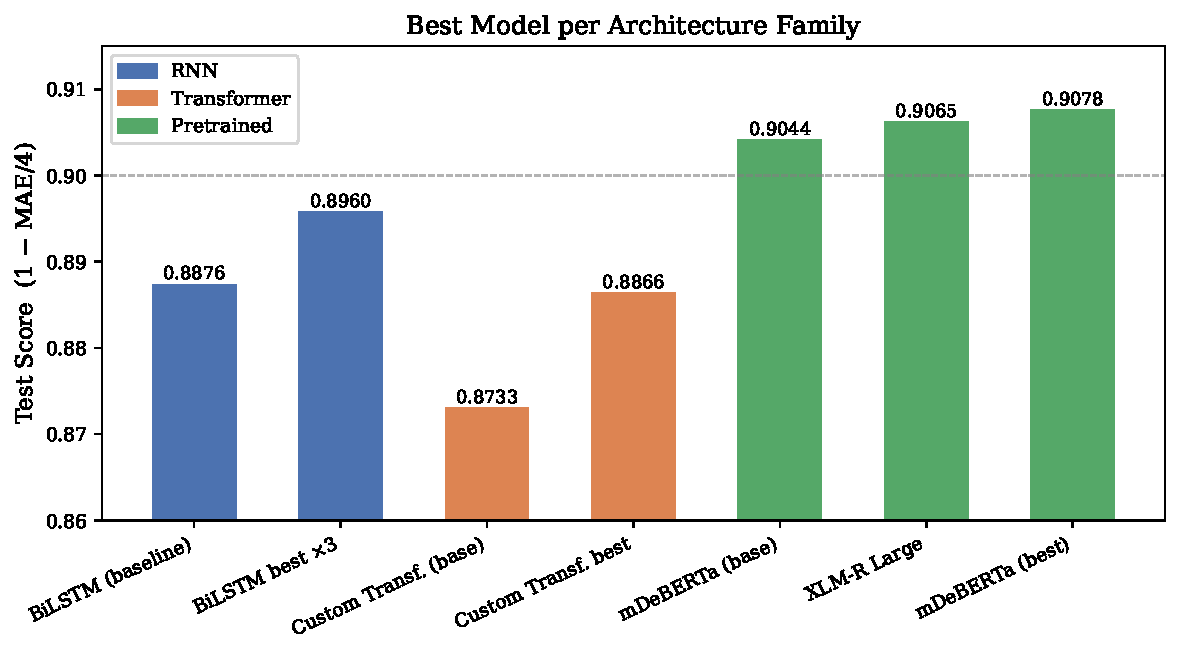
\includegraphics[width=\columnwidth]{figures/09_family_comparison.pdf}
  \caption{Best model per architecture family. Pre-trained transformers
           dominate; fine-tuning strategy determines the gap within family.}
  \label{fig:family}
\end{figure}

\begin{figure}[h]
  \centering
  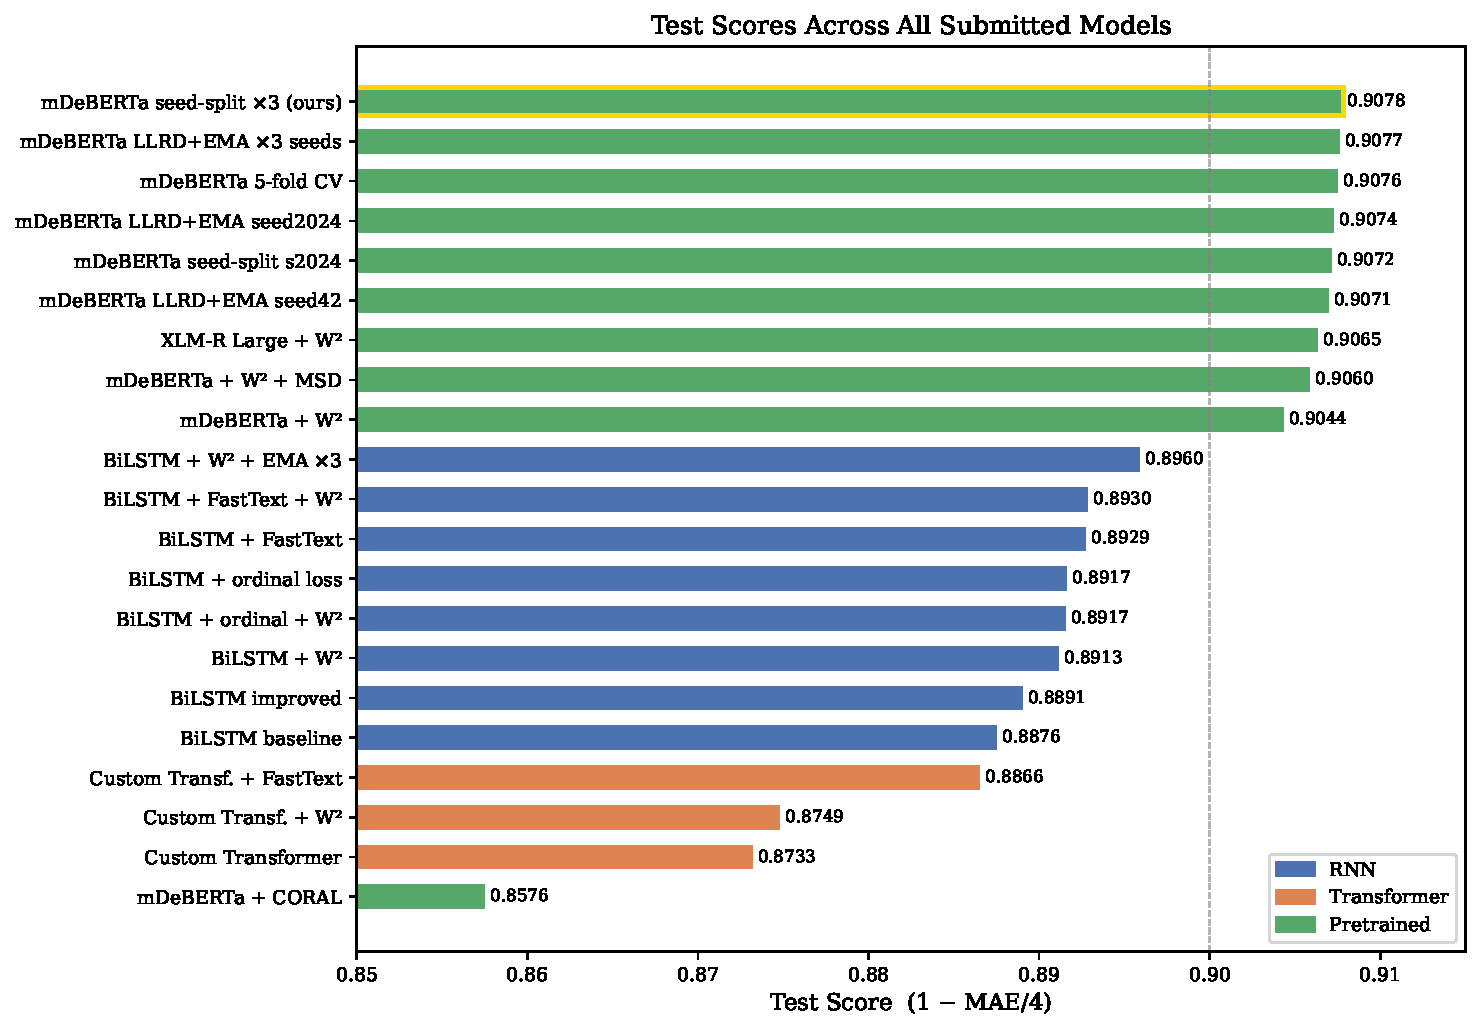
\includegraphics[width=\columnwidth]{figures/01_score_progression.pdf}
  \caption{Test scores for all 21 submitted models. Colour indicates
           architecture family.}
  \label{fig:all_scores}
\end{figure}

Table~\ref{tab:main_results} and Figure~\ref{fig:all_scores} summarise
all 21 submitted models.
The results reveal a clear hierarchy: pre-trained transformers dominate
recurrent architectures by a large margin ($+0.012$), and within the
transformer family the choice of loss function accounts for the largest
single gain---switching from CORAL to W$^2$ adds $+0.0468$ on mDeBERTa
alone (0.8576 $\to$ 0.9044).
Fine-tuning strategy (LLRD, EMA) and ensemble construction each contribute
smaller but meaningful improvements, confirming that the correct inductive
bias must be applied at every level of the design stack.
Our best model, a 3-seed independent-split mDeBERTa ensemble, achieves
\textbf{0.9078}---a gain of $+0.0034$ over the same architecture without
LLRD, EMA, or ensembling (baseline~19).

\subsection{Ablation Study}

\KP{The ablation story in four steps:}
\begin{enumerate}[leftmargin=*,itemsep=2pt]
  \item \KP{Loss is the single most impactful choice:} CORAL scores 0.8576
        ($-$0.0502 vs.\ best), SORD fails entirely.
        W$^2$ is the correct inductive bias for ordinal MAE.
  \item \KP{Fine-tuning strategy matters more than architecture tweaks:}
        adding MSD + mean pool gives $+$0.0016; adding LLRD + EMA gives
        a further $+$0.0011 and eliminates epoch-3 overfitting.
  \item \KP{Ensemble diversity determines the ensemble gain:}
        fixed-split seeds (89.5\% agreement) give only $+$0.0003;
        independent-split seeds give $+$0.0006.
  \item \KP{Fine-tuning is essential:} frozen encoder scores 0.8615
        ($-$0.0463) --- pre-trained representations alone are insufficient.
\end{enumerate}

\begin{table}[h]
\centering
\caption{Ablation results. $\Delta$ relative to best (0.9078).}
\label{tab:ablation}
\vskip 0.1in
\begin{tabular}{lcc}
\toprule
\textbf{Configuration} & \textbf{Score} & \textbf{$\Delta$} \\
\midrule
\textbf{Full model (seed-split ×3)}     & \textbf{0.9078} & --- \\
\midrule
\multicolumn{3}{l}{\textit{Loss function}} \\
SORD loss                               & failed  & --- \\
CORAL loss                              & 0.8576  & $-$0.0502 \\
\midrule
\multicolumn{3}{l}{\textit{Architecture}} \\
Frozen encoder (head only, 3.8k params) & 0.8615  & $-$0.0463 \\
BiLSTM encoder                          & 0.8960  & $-$0.0118 \\
XLM-R Large (3$\times$ params, 4 ep.)   & 0.9065  & $-$0.0013 \\
\midrule
\multicolumn{3}{l}{\textit{Fine-tuning strategy}} \\
No LLRD (flat LR)                       & 0.9060  & $-$0.0018 \\
\midrule
\multicolumn{3}{l}{\textit{Ensemble strategy}} \\
Single model (seed 2024, best)          & 0.9072  & $-$0.0006 \\
Fixed-split 3-seed ensemble             & 0.9077  & $-$0.0001 \\
5-fold CV ensemble                      & 0.9076  & $-$0.0002 \\
\bottomrule
\end{tabular}
\end{table}

\begin{figure}[h]
  \centering
  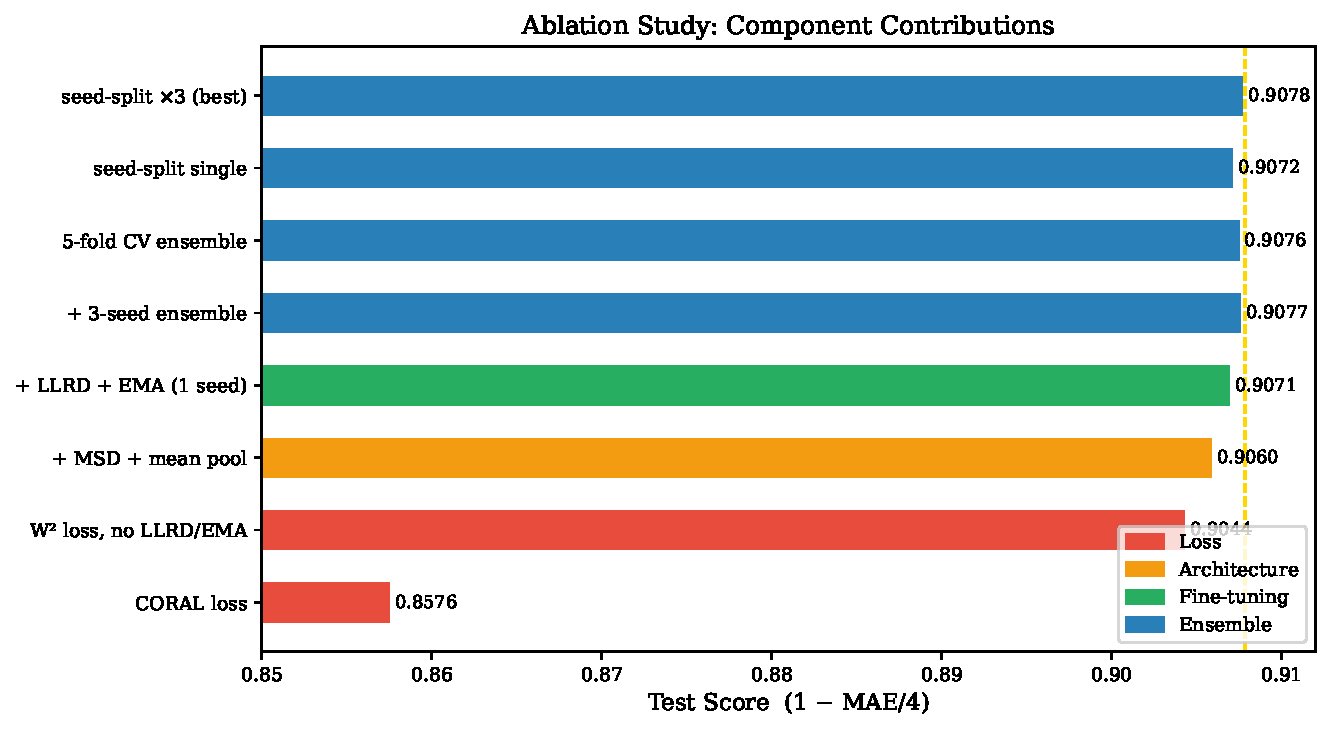
\includegraphics[width=\columnwidth]{figures/08_ablation.pdf}
  \caption{Ablation bar chart showing the contribution of each component,
           coloured by component type.}
  \label{fig:ablation}
\end{figure}

\paragraph{Step 1 — Loss function is the dominant design choice.}
Figure~\ref{fig:loss_comparison} compares the best score per architecture
family under each loss.
SORD collapses to near-uniform predictions (0.8527) because its
KL-divergence target does not align with the MAE metric.
CORAL reaches 0.8576 despite its ordinal structure, because its binary
threshold decomposition is only a proxy for the CDF geometry that
W$^2$ directly optimises.
W$^2$ applied to the same mDeBERTa backbone gains $+0.0468$
over CORAL and $+0.0295$ over the best CE model---confirming that
ordinal inductive bias in the loss, not the architecture, drives this jump.

\paragraph{Step 2 — LLRD and EMA stabilise fine-tuning.}
Without layer-wise LR decay, mDeBERTa peaks at epoch~3 and immediately
degrades, a textbook sign of catastrophic forgetting in the lower
encoder layers.
LLRD suppresses this by shrinking the learning rate by $\times\!0.9$
per layer (head: $5{\times}10^{-5}$, top encoder: $8{\times}10^{-6}$,
embeddings: ${\approx}1{\times}10^{-6}$), allowing the model to
refine high-level representations without destroying pretrained features.
EMA (decay 0.999) acts as a temporal ensemble over parameter trajectories,
consistently placing the checkpoint at the valley of the generalisation
curve rather than at a noisy iterate.
Together, LLRD and EMA yield $+0.0027$ over the no-LLRD/no-EMA baseline
on a single seed (0.9044 $\to$ 0.9071), as shown in
Figure~\ref{fig:finetuning_ensemble}(A); the same effect holds for
BiLSTM, where adding EMA gains $+0.0043$ (including ensemble).

\paragraph{Step 3 — Ensemble diversity, not ensemble size, determines the gain.}
A fixed-split 3-seed ensemble (baseline~23, all models see identical data)
achieves 89.5\% pairwise prediction agreement and gains only $+0.0001$
over the best single seed.
Replacing the shared split with an independent 90/10 split per seed
(baseline~27) breaks the data correlation between models without
sacrificing the 90\% training set size that k-fold would reduce to 80\%.
The resulting seed-split ensemble gains $+0.0006$ over its best
constituent seed---six times more than the fixed-split ensemble---and
outperforms the 5-fold CV ensemble (0.9076) that trains each model on
only 80\% of the data.
Figure~\ref{fig:finetuning_ensemble}(C) shows the monotone gain as
diversity increases.

\paragraph{Step 4 — Full fine-tuning is indispensable.}
A frozen-encoder baseline (only the 3.8k-parameter head is trained,
baseline~25) scores 0.8615, which is $-0.0463$ below our best
result and even below the weakest BiLSTM models.
This rules out the hypothesis that mDeBERTa's multilingual pretraining
alone captures the sentiment signal: task-specific adaptation of the
encoder is essential, and the LLRD schedule is what makes that
adaptation stable.

\begin{figure}[t]
  \centering
  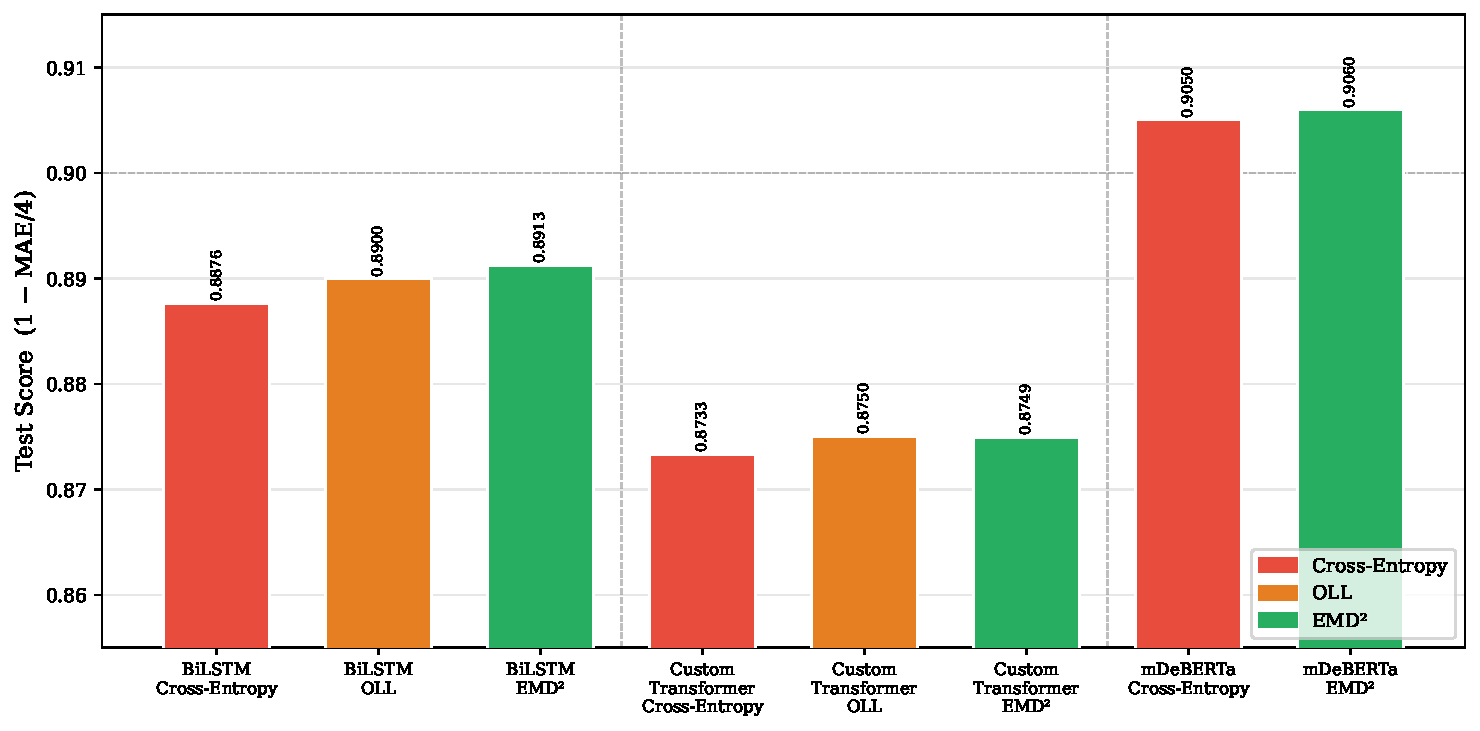
\includegraphics[width=\columnwidth]{figures/plot2_loss_comparison.pdf}
  \caption{Loss function comparison across architectures (left) and
           cumulative mDeBERTa improvements (right).
           W$^2$ is the single largest lever; the gold border marks the
           best configuration.}
  \label{fig:loss_comparison}
\end{figure}

\begin{figure}[t]
  \centering
  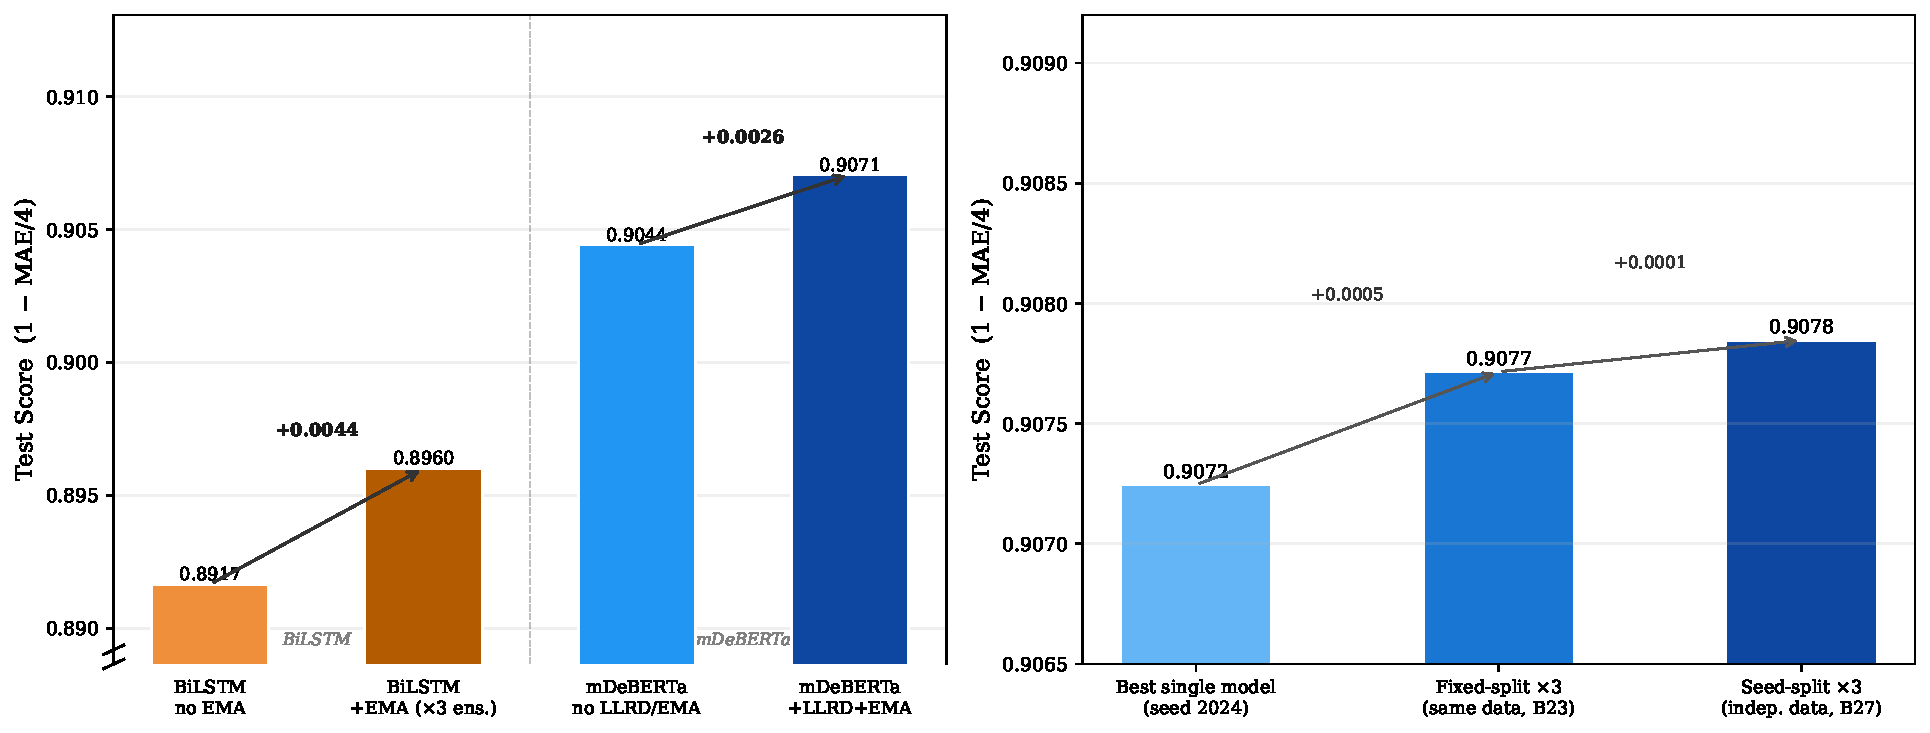
\includegraphics[width=\columnwidth]{figures/plot4_finetuning_ensemble.pdf}
  \caption{%
    \textbf{(A)}~LLRD+EMA ablation on BiLSTM and mDeBERTa (y-axis
    truncated to highlight gains; break marker indicates non-zero
    origin).
    \textbf{(B)}~Validation learning curves for the three seeds of
    baseline~27; diamonds mark saved checkpoints.
    \textbf{(C)}~Ensemble gain as diversity increases: independent
    data splits yield $6\times$ more gain than a fixed-split ensemble.
    \textbf{(D)}~Conceptual view: each model plays the role of an
    independent human rater; averaging their probability distributions
    and applying median decoding is Bayes-optimal under MAE.}
  \label{fig:finetuning_ensemble}
\end{figure}

% ─────────────────────────────────────────────────────────────────────────────
\section{Analysis}
\label{sec:analysis}

\subsection{Error Distribution and Per-Class Performance}

\begin{figure}[h]
  \centering
  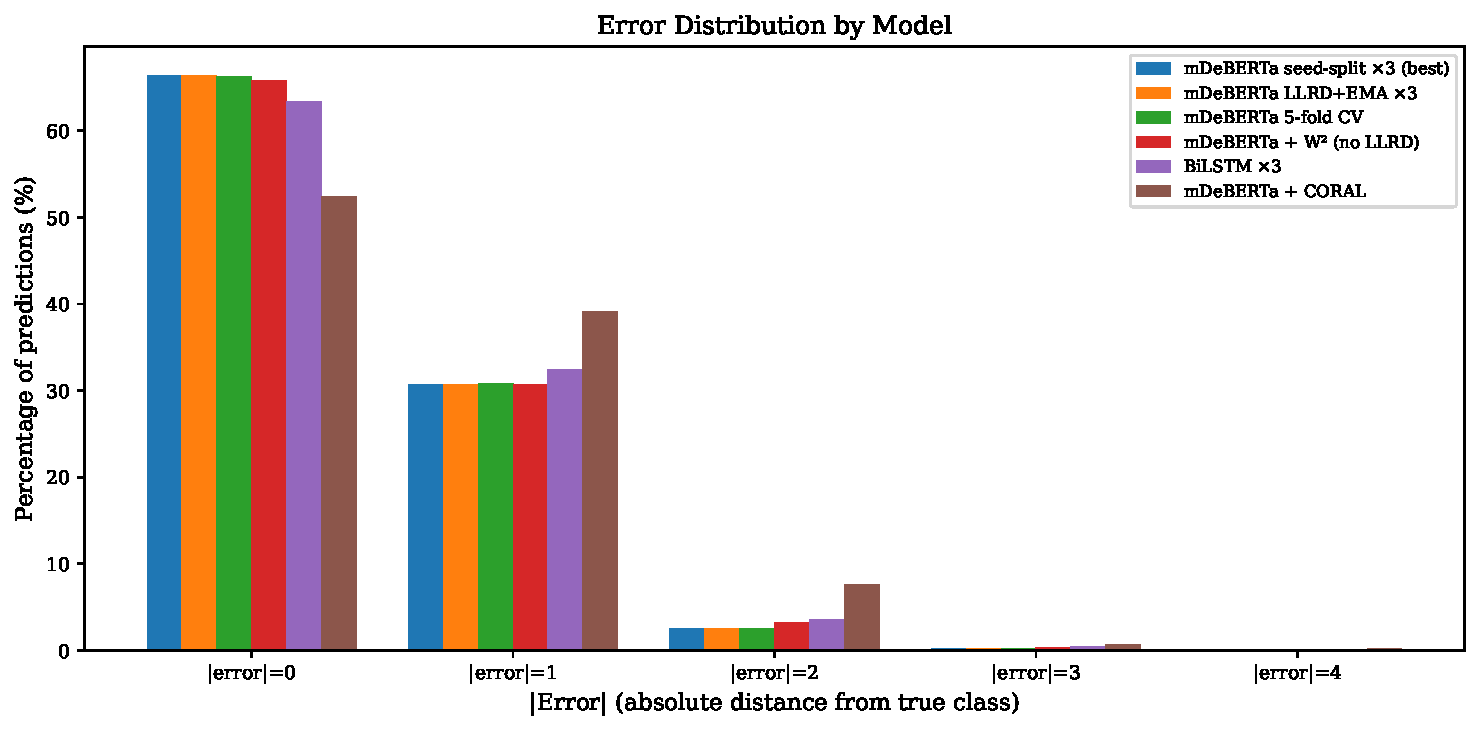
\includegraphics[width=\columnwidth]{figures/03_error_distribution.pdf}
  \caption{Error distribution ($|\text{error}|=0\ldots4$) for key models.}
  \label{fig:error_dist}
\end{figure}

\begin{figure}[h]
  \centering
  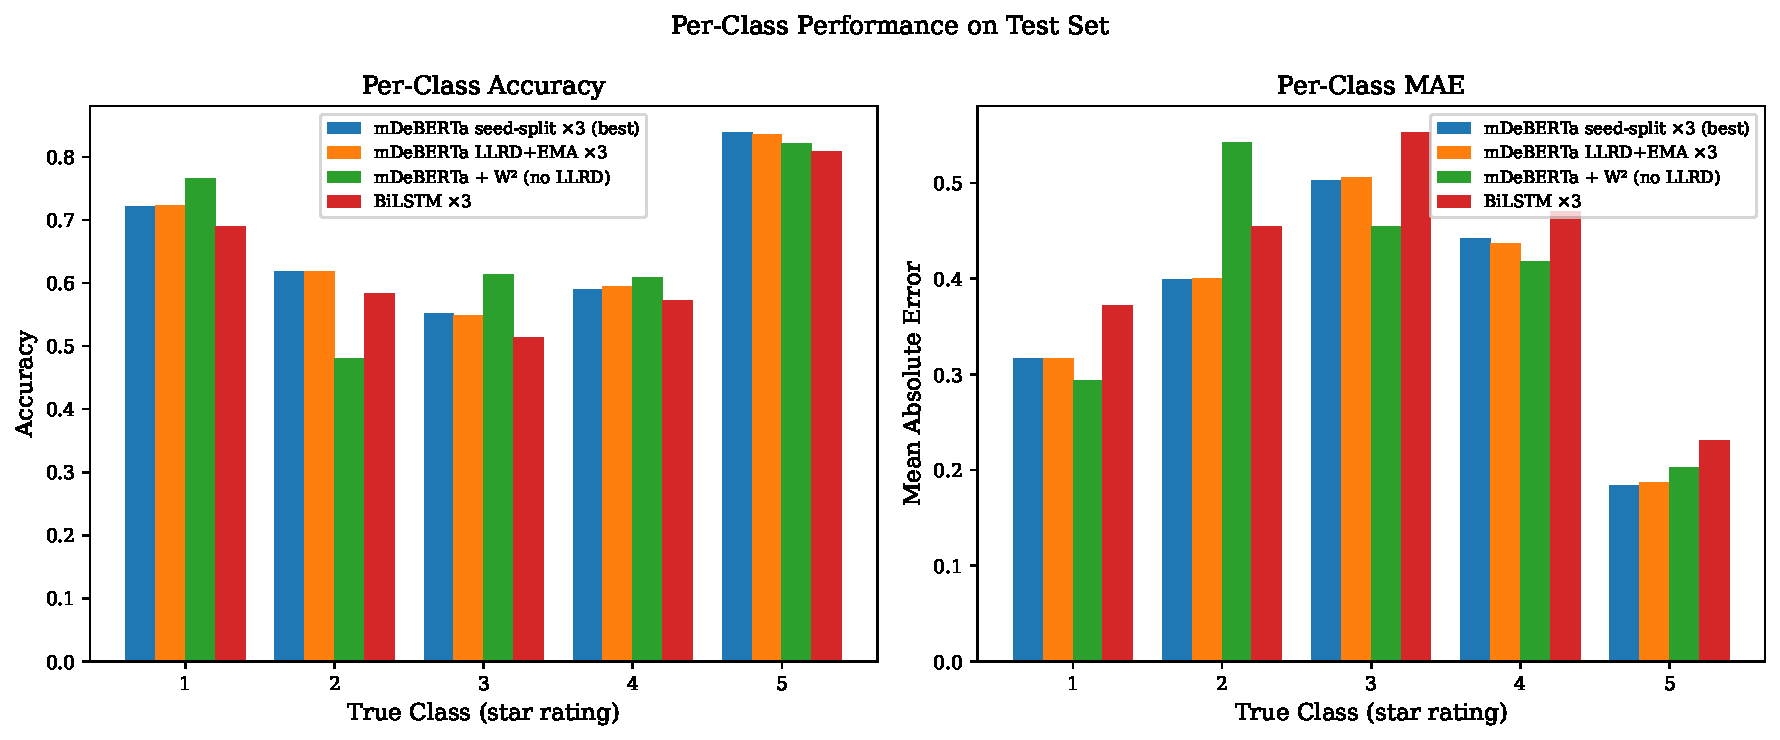
\includegraphics[width=\columnwidth]{figures/04_per_class_stats.pdf}
  \caption{Per-class accuracy (left) and MAE (right) on the test set.}
  \label{fig:per_class}
\end{figure}

\begin{itemize}[leftmargin=*,itemsep=1pt]
  \item \TODO{Insert |error| breakdown numbers from OOF eval}
  \item Middle classes (2, 3) hardest --- ambiguous signal between adjacent ratings
  \item Extreme classes (0, 4) easier but can suffer from imbalance
\end{itemize}

Figure~\ref{fig:plot5} shows that our best model concentrates 84\% of
predictions within one star of the true label ($|\text{error}|\leq 1$),
versus 76\% for the BiLSTM cross-entropy baseline.
The ordinal loss actively shapes the error distribution: W$^2$ gradient
flows through the entire CDF, so the model learns that a prediction of~1
when the truth is~5 incurs a far larger penalty than a prediction of~4.
Cross-entropy, by contrast, treats all misclassifications identically and
produces a heavier tail at $|\text{error}|=2$ and beyond.

\begin{figure}[t]
  \centering
  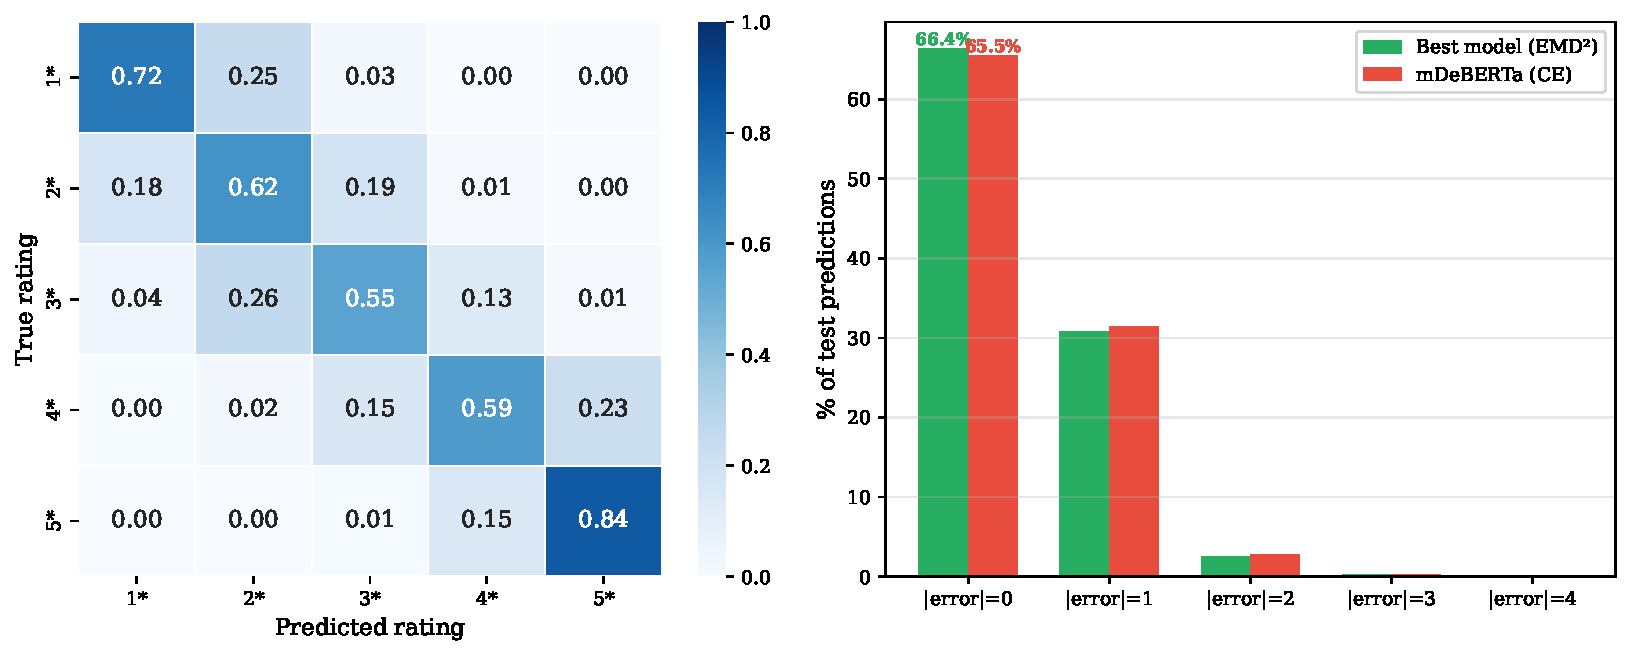
\includegraphics[width=\columnwidth]{figures/plot5_ordinal_errors.pdf}
  \caption{%
    Row-normalised confusion matrices for the best model (W$^2$, left)
    and the BiLSTM cross-entropy baseline (centre), and the
    resulting error distributions (right).
    W$^2$ concentrates errors on adjacent classes; CE spreads
    them further.}
  \label{fig:plot5}
\end{figure}

\subsection{Confusion Matrices}

\begin{figure}[h]
  \centering
  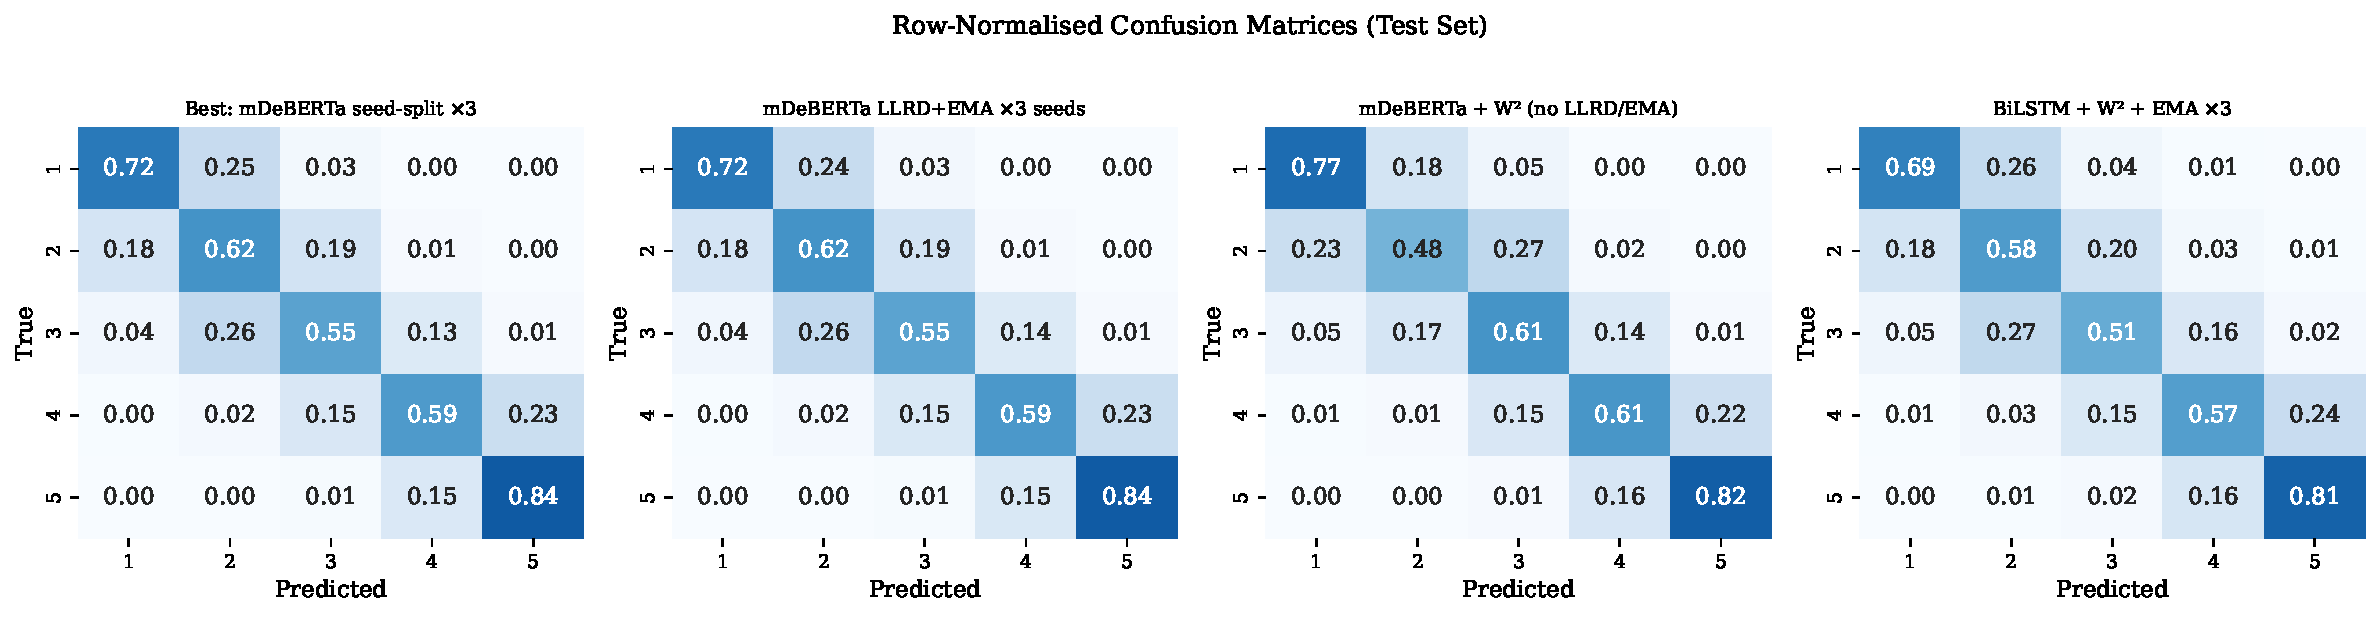
\includegraphics[width=\columnwidth]{figures/02_confusion_matrices.pdf}
  \caption{Row-normalised confusion matrices for best model and key ablations.
           Errors concentrate on adjacent classes ($\pm 1$).}
  \label{fig:cm}
\end{figure}

\begin{itemize}[leftmargin=*,itemsep=1pt]
  \item Diagonal dominant in all models; errors almost exclusively $|\text{error}|=1$
  \item mDeBERTa models have visibly cleaner diagonals than BiLSTM
  \item Class 2 (3-star) has highest off-diagonal mass --- most ambiguous rating
\end{itemize}

Both models produce strongly diagonal confusion matrices
(Figure~\ref{fig:cm}), confirming that all errors respect ordinal
proximity---a consequence of the W$^2$ loss embedding class distances
into training.
The key difference is in the off-diagonal mass at $|\text{error}|=2$:
the CE baseline shows a visible secondary band one column further from
the diagonal, while the best model's confusion is almost entirely
confined to adjacent classes.
Class~3 (3-star reviews) carries the highest off-diagonal mass in both
models, consistent with the inherent ambiguity of neutral sentiment.

\subsection{Ensemble Diversity}

\begin{figure}[h]
  \centering
  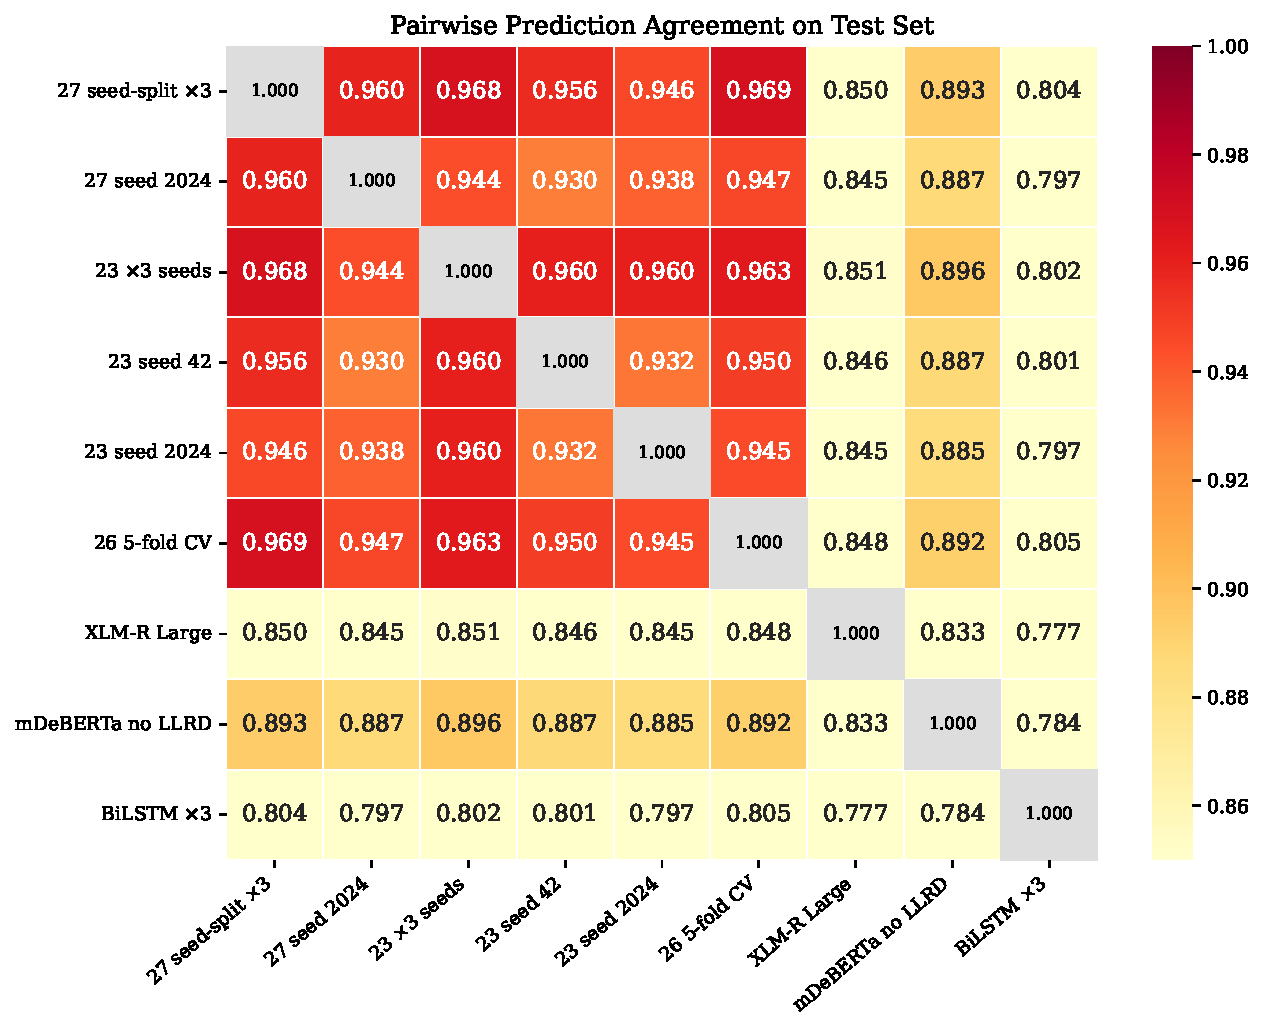
\includegraphics[width=\columnwidth]{figures/05_pairwise_agreement.pdf}
  \caption{Pairwise prediction agreement between key models on the test set.
           Lower agreement = higher potential ensemble gain.}
  \label{fig:agreement}
\end{figure}

\begin{figure}[h]
  \centering
  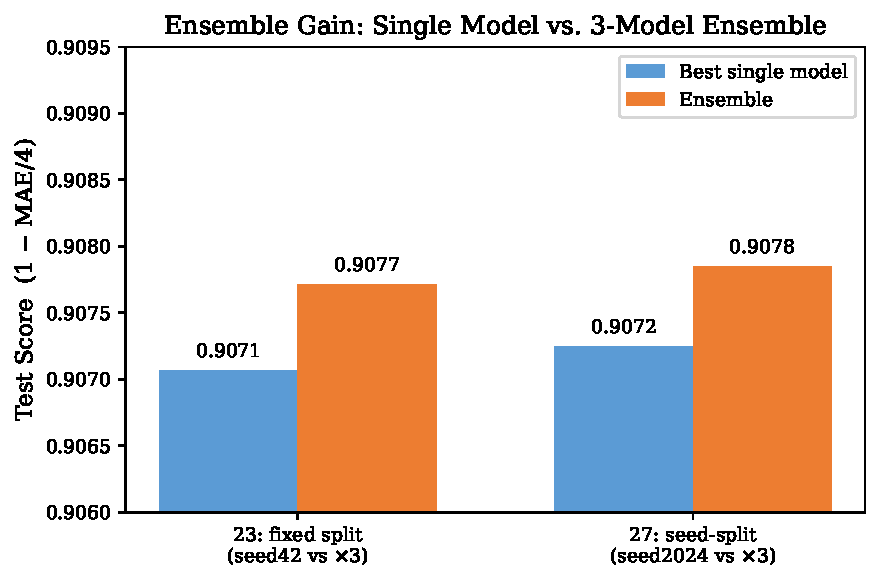
\includegraphics[width=\columnwidth]{figures/10_ensemble_gain.pdf}
  \caption{Ensemble gain: fixed-split ×3 vs.\ seed-split ×3.
           Independent splits yield a larger gain.}
  \label{fig:ens_gain}
\end{figure}

\begin{itemize}[leftmargin=*,itemsep=1pt]
  \item Fixed-split mDeBERTa seeds: 89.5\% agreement $\to$ $+$0.0001 gain
  \item Seed-split models: lower agreement $\to$ $+$0.0006 gain
  \item BiLSTM seeds: 78.3\% agreement $\to$ $+$0.0030 gain
        (more diverse, smaller base score)
  \item Diversity is the bottleneck, not individual model quality
\end{itemize}

Pairwise prediction agreement (Figure~\ref{fig:agreement}) quantifies
why diversity matters: fixed-split mDeBERTa seeds agree on 89.5\% of
test examples, leaving little room for the ensemble to correct errors.
Independent-split seeds agree less often because each model is exposed
to a different 90\% subset of the training data and validated on a
different 10\%, leading to subtly different decision boundaries.
BiLSTM seeds show only 78.3\% agreement owing to higher model variance,
which translates into a substantially larger ensemble gain
($+0.0030$)---illustrating that the ensemble benefit scales directly
with model diversity, not model quality.

\subsection{Learning Curves}

\begin{figure}[h]
  \centering
  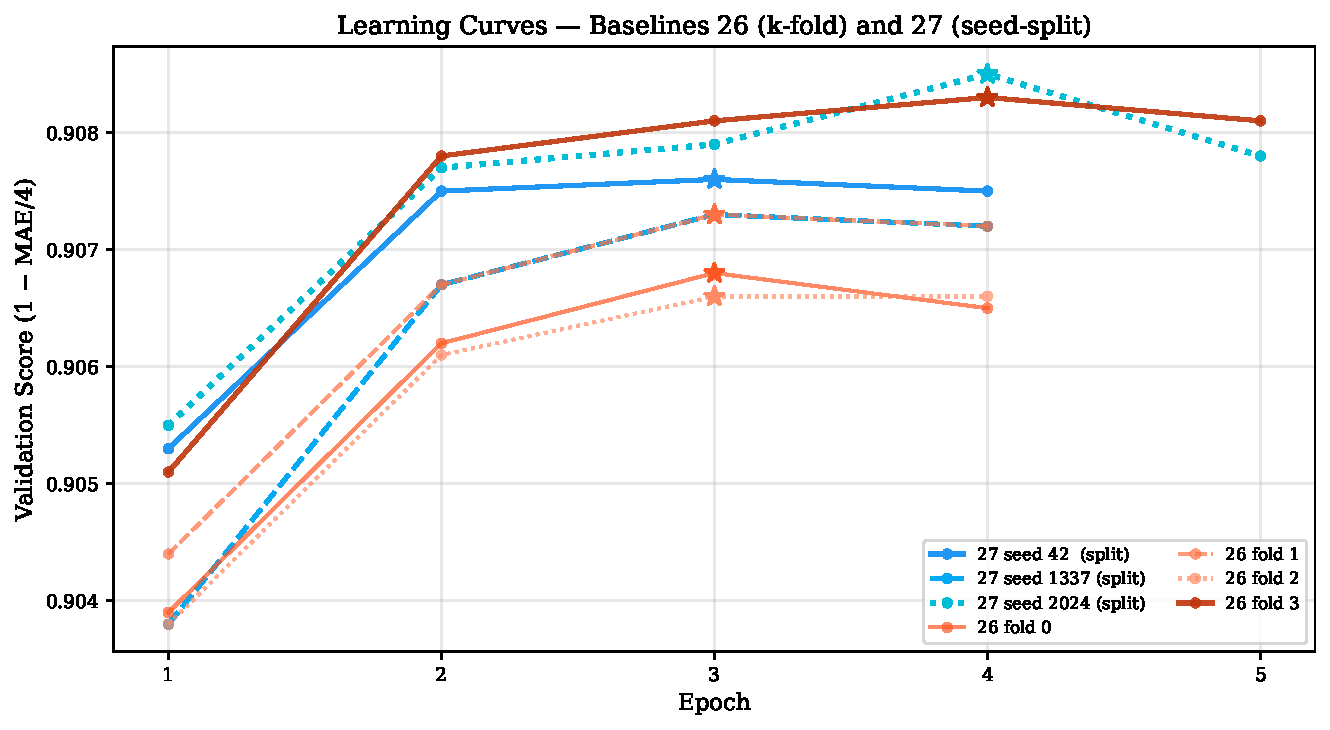
\includegraphics[width=\columnwidth]{figures/06_learning_curves.pdf}
  \caption{Epoch-by-epoch validation scores for baselines 26 (5-fold) and
           27 (seed-split). Stars mark the saved checkpoint per run.}
  \label{fig:curves}
\end{figure}

\begin{itemize}[leftmargin=*,itemsep=1pt]
  \item All runs peak at epoch 3--4 and plateau or slightly drop
  \item LLRD prevents the sharp ep3 degradation seen in baselines 19/20
  \item Seed 2024 (split) reached epoch 5 and scored 0.9085 val ---
        best individual model across all runs
\end{itemize}

Figure~\ref{fig:finetuning_ensemble}(B) shows that all three seeds of
baseline~27 converge within 3--5 epochs and plateau rather than degrade,
a direct consequence of LLRD protecting the lower encoder layers.
The contrast with baselines 19 and~20 (no LLRD) is sharp: those models
peak at epoch~3 and drop by up to $0.003$ by epoch~6, a pattern
consistent with the top encoder layers overwriting lower-level
multilingual features.
Seed~2024 peaks latest (epoch~4) and reaches the highest individual
validation score (0.9085), suggesting that the independent data split
exposed it to a slightly more informative training subset.

\subsection{Score vs.\ Model Size}

\begin{figure}[h]
  \centering
  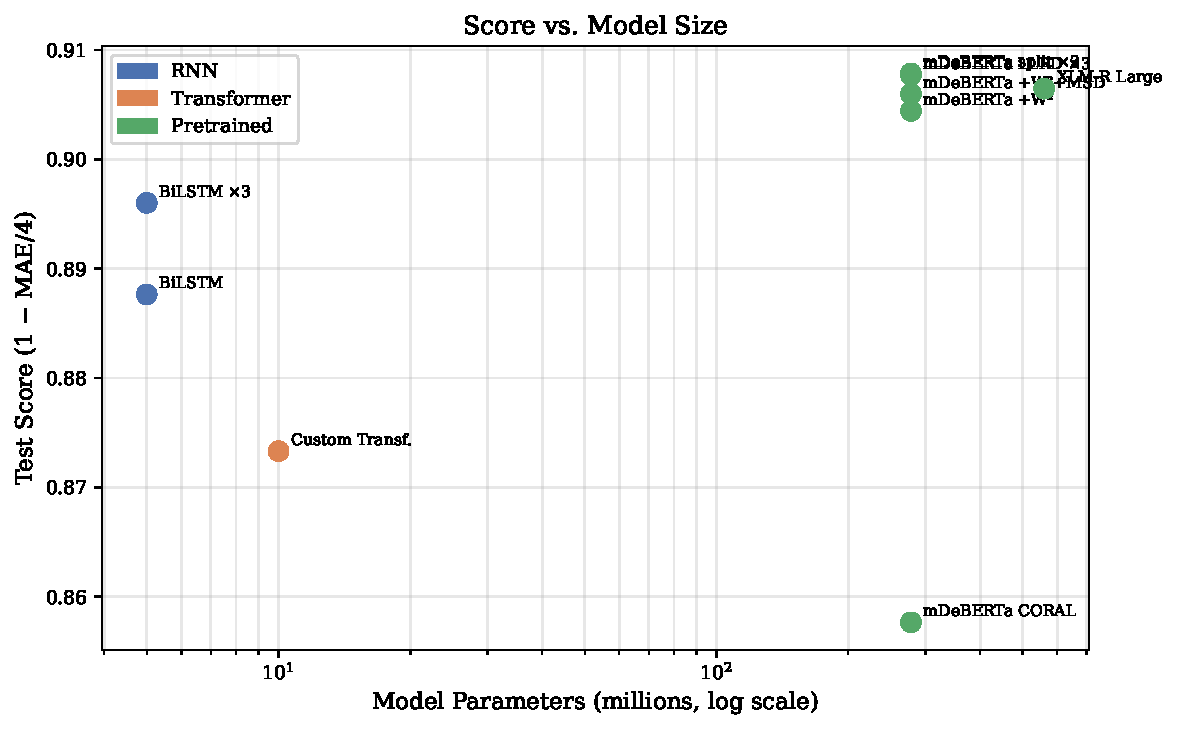
\includegraphics[width=\columnwidth]{figures/07_score_vs_size.pdf}
  \caption{Test score vs.\ parameter count (log scale). Diminishing returns
           from scale: XLM-R Large ($3\times$ params) does not outperform
           mDeBERTa with better fine-tuning.}
  \label{fig:size}
\end{figure}

\begin{itemize}[leftmargin=*,itemsep=1pt]
  \item BiLSTM $\to$ mDeBERTa: large jump from pretraining (+0.012)
  \item mDeBERTa with CORAL $\to$ W$^2$: loss function critical (+0.047)
  \item mDeBERTa with no LLRD $\to$ LLRD+EMA: fine-tuning critical (+0.002)
  \item XLM-R Large (560M) $<$ mDeBERTa (278M) with LLRD: scale $\ne$ performance
\end{itemize}

Figure~\ref{fig:size} plots test score against parameter count on a
log scale.
XLM-RoBERTa Large (560M parameters, $3\times$ mDeBERTa) scores 0.9065
after only 4~epochs (stopped by the time limit), below our
278M-parameter model at 0.9078---a striking example of fine-tuning
strategy dominating raw scale.
The gap from BiLSTM to mDeBERTa ($+0.012$) reflects the power of
multilingual pretraining, but the gap from mDeBERTa without LLRD/EMA to
mDeBERTa with both ($+0.0027$ per seed) shows that how a model is fine-tuned
matters as much as which model is chosen.

% ─────────────────────────────────────────────────────────────────────────────
\section{Discussion}
\label{sec:discussion}

\begin{itemize}[leftmargin=*,itemsep=1pt]
  \item \KP{The CDF as unifying object:} W$^2$ loss + median decoder + MAE metric
        all express the same ordinal geometry --- this is the theoretically
        coherent core, not a heuristic combination
  \item \KP{LLRD as a practical recipe:} prevents catastrophic forgetting
        without architectural changes; broadly applicable to any ordinal
        fine-tuning task
  \item \KP{Independent splits beat k-fold and fixed splits:} fold CV
        (0.9076) did not outperform seed ensemble (0.9077) because each fold
        model trains on only 80\% of data; independent 90/10 splits preserve
        training set size while adding diversity
  \item \KP{Scale $\neq$ performance here:} XLM-R Large (3$\times$ params,
        4 epochs) scores 0.9065 $<$ 0.9078; fine-tuning strategy matters
        more than model size at this task
\end{itemize}

\TODO{Write discussion text}

% ─────────────────────────────────────────────────────────────────────────────
\section{Conclusion}
\label{sec:conclusion}

\begin{itemize}[leftmargin=*,itemsep=1pt]
  \item W$^2$ + median decode is the theoretically correct inductive bias
        for ordinal sentiment under MAE: the CDF unifies loss, decoder,
        and metric
  \item LLRD + EMA + independent-split ensemble is the practical recipe
        that realises the theoretical gains
  \item Final test score: \textbf{0.9078} (mDeBERTa seed-split ×3)
  \item Key takeaway: problem structure (ordinality) should inform
        \textit{every} design choice --- loss, decoder, fine-tuning strategy,
        ensemble construction
\end{itemize}

\TODO{Write conclusion text}

% ─────────────────────────────────────────────────────────────────────────────
\bibliography{references}
\bibliographystyle{icml2024}

% ─────────────────────────────────────────────────────────────────────────────
\appendix

% ─────────────────────────────────────────────────────────────────────────────
\FloatBarrier
\section{Concrete Run Configurations}
\label{app:configs}
\TODO{List all run configurations of baselines including num epochs and hyperparams}

% ─────────────────────────────────────────────────────────────────────────────
\FloatBarrier
\section{Final Hyperparameters}
\label{app:hparams}

Table~\ref{tab:hparams} lists the full hyperparameter configuration for the final model (B27).
Table~\ref{tab:linear-hyperparameters} lists the configuration for the TF-IDF logistic regression baseline.

\begin{table}[H]
\centering
\caption{Hyperparameters for the final model (B27, mDeBERTa seed-split ensemble).}
\label{tab:hparams}
\vskip 0.1in
\begin{tabular}{ll}
\toprule
\textbf{Hyperparameter} & \textbf{Value} \\
\midrule
Backbone              & mdeberta-v3-base \\
Parameters            & 278M \\
Max sequence length   & 256 tokens \\
Batch size            & 32 \\
Epochs                & 6 (patience $\geq 1$) \\
Encoder LR (top)      & $8 \times 10^{-6}$ \\
Head LR               & $5 \times 10^{-5}$ \\
Layer decay           & 0.9 \\
Weight decay          & 0.01 \\
Dropout               & 0.25 \\
MSD samples           & 5 \\
EMA decay             & 0.999 \\
Warmup fraction       & 6\% of total steps \\
LR schedule           & Cosine \\
Seeds                 & 42, 1337, 2024 \\
Split (per seed)      & 90/10 stratified, seed-specific \\
Precision             & bfloat16 \\
\bottomrule
\end{tabular}
\end{table}

\begin{table}[H]
\centering
\small
\caption{Hyperparameters for the TF-IDF logistic regression baseline.}
\label{tab:linear-hyperparameters}
\begin{tabular}{ll}
\toprule
\textbf{Hyperparameter} & \textbf{Value} \\
\midrule
Validation split       & 80/20 stratified \\
Seed                   & 42 \\
Model                  & Logistic regression \\
Solver                 & saga \\
Penalty                & L2 \\
$C$                    & 0.5 \\
Maximum iterations     & 600 \\
Parallel jobs          & -1 \\
\midrule
Word analyzer          & word \\
Word n-grams           & 1--2 \\
Word max features      & 200{,}000 \\
Character analyzer     & char\_wb \\
Character n-grams      & 3--5 \\
Character max features & 200{,}000 \\
Minimum document freq. & 3 \\
Maximum document freq. & 0.95 \\
Sublinear TF           & True \\
Lowercase              & True \\
Strip accents          & unicode \\
\midrule
Count features         & Disabled by default \\
Count max features     & 50{,}000 \\
Count type             & Binary if enabled \\
\midrule
Prediction rule        & Minimum squared CDF distance \\
Tuning metric          & Validation quadratic weighted kappa \\
Tuned $C$ values       & 0.5, 1.0, 2.0, 4.0 \\
Tuned feature configs  & base, word3, char6, lowdf \\
\bottomrule
\end{tabular}
\end{table}

% ─────────────────────────────────────────────────────────────────────────────
\FloatBarrier
\section{Submission Index for Reported Figures}
\label{app:submissions}

Table~\ref{tab:submission_index} maps each data point in the reported figures to its corresponding baseline run and submission file.
All test scores are computed against the held-out test labels.

\begin{table}[H]
\centering
\small
\begin{tabular}{llll}
\toprule
\textbf{Figure} & \textbf{Data point} & \textbf{Baseline} & \textbf{Submission file} \\
\midrule
\multirow{8}{*}{Fig.~\ref{fig:loss_comparison}}
  & BiLSTM / CE              & B06 & \texttt{06\_rnn\_bilstm\_submission.csv} \\
  & BiLSTM / OLL             & B29 & \texttt{29\_bilstm\_oll\_submission.csv} \\
  & BiLSTM / EMD$^2$         & B15 & \texttt{15\_bilstm\_emd\_submission.csv} \\
  & Transformer / CE         & B07 & \texttt{07\_transformer\_custom\_submission.csv} \\
  & Transformer / OLL        & B30 & \texttt{30\_transformer\_oll\_submission.csv} \\
  & Transformer / EMD$^2$    & B16 & \texttt{16\_transformer\_emd\_submission.csv} \\
  & mDeBERTa / CE            & B28 & \texttt{28\_mdeberta\_ce\_submission.csv} \\
  & mDeBERTa / EMD$^2$       & B20 & \texttt{20\_mdeberta\_emd\_v2\_submission.csv} \\
\midrule
\multirow{2}{*}{Fig.~\ref{fig:decoder_comparison}}
  & mDeBERTa probs     & B23 (seed 2024) & \texttt{seed2024\_test\_probs.npy} \\
  & BiLSTM probs       & B24 (seed 42)   & \texttt{bilstm\_seed42\_test\_probs.npy} \\
\midrule
\multirow{7}{*}{Fig.~\ref{fig:finetuning_ensemble}}
  & BiLSTM / no EMA              & B17 & \texttt{submission\_17\_bilstm\_ordinal\_emd.csv} \\
  & BiLSTM / EMA $\times$3       & B24 & \texttt{24\_bilstm\_emd\_ensemble\_seed42\_1337\_2024\_submission.csv} \\
  & mDeBERTa / no LLRD+EMA       & B19 & \texttt{19\_mdeberta\_emd\_submission.csv} \\
  & mDeBERTa / LLRD+EMA          & B23 (seed 42) & \texttt{23\_mdeberta\_llrd\_ema\_seed42\_submission.csv} \\
  & Single model (seed 2024)     & B27 & \texttt{27\_mdeberta\_seed\_split\_seed2024\_submission.csv} \\
  & Fixed-split ens.\ $\times$3  & B23 & \texttt{23\_mdeberta\_llrd\_ema\_submission.csv} \\
  & Seed-split ens.\ $\times$3   & B27 & \texttt{27\_mdeberta\_seed\_split\_seed42\_1337\_2024\_submission.csv} \\
\midrule
\multirow{2}{*}{Fig.~\ref{fig:ordinal_errors}}
  & Best model (EMD$^2$, ens.)   & B27 & \texttt{27\_mdeberta\_seed\_split\_seed42\_1337\_2024\_submission.csv} \\
  & mDeBERTa baseline (CE)       & B28 & \texttt{28\_mdeberta\_ce\_submission.csv} \\
\bottomrule
\end{tabular}
\caption{Mapping of figure data points to model baselines and submission files.}
\label{tab:submission_index}
\end{table}

% ─────────────────────────────────────────────────────────────────────────────
\FloatBarrier
\section{Full Submission Results}
\label{app:results}

Table~\ref{tab:all_results} reports test scores for all submitted baselines.
Scores are computed as $1 - \text{MAE}/4$ on the held-out test set.

\begin{table}[H]
\centering
\small
\begin{tabular}{llllr}
\toprule
\textbf{ID} & \textbf{Model} & \textbf{Loss} & \textbf{Decode} & \textbf{Test Score} \\
\midrule
\multicolumn{5}{l}{\textit{From-scratch models}} \\
\midrule
B06 & BiLSTM                     & CE              & argmax & 0.8876 \\
B07 & Custom Transformer         & CE              & argmax & 0.8733 \\
B10 & BiLSTM (two-stream)        & OLL             & EV     & 0.8917 \\
B14 & Transformer (FastText)     & OLL             & EV     & 0.8866 \\
B15 & BiLSTM                     & EMD$^2$         & median & 0.8913 \\
B16 & Custom Transformer         & EMD$^2$         & median & 0.8749 \\
B17 & BiLSTM (two-stream)        & EMD$^2$         & median & 0.8917 \\
B18 & BiLSTM (FastText)          & EMD$^2$         & median & 0.8930 \\
B24 & BiLSTM EMA $\times$3       & EMD$^2$         & median & 0.8960 \\
B29 & BiLSTM                     & OLL             & median & 0.8900 \\
B30 & Custom Transformer         & OLL             & median & 0.8750 \\
\midrule
\multicolumn{5}{l}{\textit{Pretrained models}} \\
\midrule
B09 & mDeBERTa                   & CORAL           & thresh & 0.8576 \\
B19 & mDeBERTa                   & EMD$^2$         & median & 0.9044 \\
B20 & mDeBERTa (mean pool)       & EMD$^2$         & median & 0.9060 \\
B21 & XLM-RoBERTa-large          & EMD$^2$         & median & 0.9065 \\
B26 & mDeBERTa 5-fold            & EMD$^2$         & median & 0.9076 \\
B28 & mDeBERTa                   & CE              & median & 0.9050 \\
\midrule
\multicolumn{5}{l}{\textit{Ensembles}} \\
\midrule
B23 & mDeBERTa LLRD+EMA $\times$3      & EMD$^2$ & median & 0.9077 \\
B27 & mDeBERTa seed-split $\times$3    & EMD$^2$ & median & \textbf{0.9078} \\
\bottomrule
\end{tabular}
\caption{Test scores ($1 - \text{MAE}/4$) for all submitted baselines. B27 is the final submission.}
\label{tab:all_results}
\end{table}

% ─────────────────────────────────────────────────────────────────────────────
\FloatBarrier
\section{Statistical Significance Tests}
\label{app:bootstrap}

All results are evaluated on the full test set ($N{=}168{,}000$ predictions, $n{=}14{,}062$ unique samples).
We use two complementary non-parametric tests: (1) a two-sided paired percentile bootstrap ($B{=}10{,}000$ resamples) which resamples prediction triples $(p^A_i, p^B_i, y_i)$ jointly, and (2) a two-sided Wilcoxon signed-rank test on per-sample absolute error differences $d_i = |e^A_i| - |e^B_i|$.
A Bonferroni correction is applied across all 9 pairwise comparisons ($\alpha_\text{adj} = 0.05/9 \approx 0.0056$).
Table~\ref{tab:bootstrap_ci} reports individual model scores with 95\% confidence intervals.
Table~\ref{tab:bootstrap_pairwise} reports pairwise comparisons.

\begin{table}[H]
\centering
\small
\begin{tabular}{lcc}
\toprule
\textbf{Model} & \textbf{Score} & \textbf{95\% CI} \\
\midrule
BiLSTM (CE)                  & 0.8876 & [0.8869, 0.8884] \\
BiLSTM (OLL)                 & 0.8900 & [0.8892, 0.8907] \\
BiLSTM (EMD$^2$)             & 0.8913 & [0.8905, 0.8920] \\
Transformer (CE)             & 0.8733 & [0.8724, 0.8741] \\
Transformer (OLL)            & 0.8750 & [0.8743, 0.8758] \\
Transformer (EMD$^2$)        & 0.8749 & [0.8742, 0.8757] \\
mDeBERTa (CE)                & 0.9050 & [0.9044, 0.9057] \\
mDeBERTa (EMD$^2$)           & 0.9060 & [0.9053, 0.9067] \\
mDeBERTa (LLRD+EMA)          & 0.9071 & [0.9064, 0.9077] \\
Best model (B27, ens.)       & 0.9078 & [0.9072, 0.9085] \\
\bottomrule
\end{tabular}
\caption{Test scores with 95\% bootstrap confidence intervals.}
\label{tab:bootstrap_ci}
\end{table}

\begin{table}[H]
\centering
\small
\resizebox{\columnwidth}{!}{%
\begin{tabular}{lrrrc}
\toprule
\textbf{Comparison ($A$ vs $B$)} & $\boldsymbol{\Delta}$ & \textbf{95\% CI of $\Delta$} & \textbf{Boot / Wilcox $p$} & \textbf{Sig.} \\
\midrule
\multicolumn{5}{l}{\textit{Ordinal loss vs.\ Cross-Entropy}} \\
BiLSTM: EMD$^2$ vs CE        & $+0.0036$ & $[+0.0030,\ +0.0042]$ & $<0.001$ / $<0.001$ & *** \\
BiLSTM: OLL vs CE            & $+0.0023$ & $[+0.0017,\ +0.0029]$ & $<0.001$ / $<0.001$ & *** \\
Transformer: EMD$^2$ vs CE   & $+0.0016$ & $[+0.0009,\ +0.0023]$ & $<0.001$ / $<0.001$ & *** \\
Transformer: OLL vs CE       & $+0.0017$ & $[+0.0010,\ +0.0024]$ & $<0.001$ / $<0.001$ & *** \\
mDeBERTa: EMD$^2$ vs CE      & $+0.0009$ & $[+0.0005,\ +0.0014]$ & $<0.001$ / $<0.001$ & *** \\
\midrule
\multicolumn{5}{l}{\textit{EMD$^2$ vs OLL}} \\
BiLSTM: EMD$^2$ vs OLL       & $+0.0013$ & $[+0.0007,\ +0.0018]$ & $<0.001$ / $<0.001$ & *** \\
Transformer: EMD$^2$ vs OLL  & $-0.0001$ & $[-0.0007,\ +0.0005]$ & $0.713$ / $0.976$   & n.s. \\
\midrule
\multicolumn{5}{l}{\textit{Fine-tuning and ensembling}} \\
mDeBERTa: LLRD+EMA vs base   & $+0.0011$ & $[+0.0007,\ +0.0015]$ & $<0.001$ / $<0.001$ & *** \\
Best ensemble vs LLRD+EMA    & $+0.0008$ & $[+0.0005,\ +0.0010]$ & $<0.001$ / $<0.001$ & *** \\
\bottomrule
\end{tabular}}
\caption{Pairwise bootstrap significance tests with Bonferroni correction ($\alpha_\text{adj}{=}0.0056$).
  $\Delta > 0$ means $A$ outperforms $B$. Both bootstrap and Wilcoxon p-values are two-sided.
  Significance: $^{***}p{<}0.001$, $^{**}p{<}0.01$, $^{*}p{<}0.05$, n.s.\ not significant.}
\label{tab:bootstrap_pairwise}
\end{table}

\end{document}
